\documentclass[,acmart]{apa6}
\usepackage{lmodern}
\usepackage{amssymb,amsmath}
\usepackage{ifxetex,ifluatex}
\usepackage{fixltx2e} % provides \textsubscript
\ifnum 0\ifxetex 1\fi\ifluatex 1\fi=0 % if pdftex
  \usepackage[T1]{fontenc}
  \usepackage[utf8]{inputenc}
\else % if luatex or xelatex
  \ifxetex
    \usepackage{mathspec}
  \else
    \usepackage{fontspec}
  \fi
  \defaultfontfeatures{Ligatures=TeX,Scale=MatchLowercase}
\fi
% use upquote if available, for straight quotes in verbatim environments
\IfFileExists{upquote.sty}{\usepackage{upquote}}{}
% use microtype if available
\IfFileExists{microtype.sty}{%
\usepackage{microtype}
\UseMicrotypeSet[protrusion]{basicmath} % disable protrusion for tt fonts
}{}
\usepackage{hyperref}
\hypersetup{unicode=true,
            pdftitle={Exploring predictors of achievement in online science classes},
            pdfborder={0 0 0},
            breaklinks=true}
\urlstyle{same}  % don't use monospace font for urls
\usepackage{graphicx,grffile}
\makeatletter
\def\maxwidth{\ifdim\Gin@nat@width>\linewidth\linewidth\else\Gin@nat@width\fi}
\def\maxheight{\ifdim\Gin@nat@height>\textheight\textheight\else\Gin@nat@height\fi}
\makeatother
% Scale images if necessary, so that they will not overflow the page
% margins by default, and it is still possible to overwrite the defaults
% using explicit options in \includegraphics[width, height, ...]{}
\setkeys{Gin}{width=\maxwidth,height=\maxheight,keepaspectratio}
\IfFileExists{parskip.sty}{%
\usepackage{parskip}
}{% else
\setlength{\parindent}{0pt}
\setlength{\parskip}{6pt plus 2pt minus 1pt}
}
\setlength{\emergencystretch}{3em}  % prevent overfull lines
\providecommand{\tightlist}{%
  \setlength{\itemsep}{0pt}\setlength{\parskip}{0pt}}
\setcounter{secnumdepth}{0}
% Redefines (sub)paragraphs to behave more like sections
\ifx\paragraph\undefined\else
\let\oldparagraph\paragraph
\renewcommand{\paragraph}[1]{\oldparagraph{#1}\mbox{}}
\fi
\ifx\subparagraph\undefined\else
\let\oldsubparagraph\subparagraph
\renewcommand{\subparagraph}[1]{\oldsubparagraph{#1}\mbox{}}
\fi

%%% Use protect on footnotes to avoid problems with footnotes in titles
\let\rmarkdownfootnote\footnote%
\def\footnote{\protect\rmarkdownfootnote}


  \title{Exploring predictors of achievement in online science classes}
    \author{\textsuperscript{}}
    \date{}
  
\shorttitle{Predictors of achievement}
\affiliation{
\vspace{0.5cm}
\textsuperscript{} }
\keywords{\newline\indent Word count: }
\usepackage{csquotes}
\usepackage{upgreek}
\captionsetup{font=singlespacing,justification=justified}

\usepackage{longtable}
\usepackage{lscape}
\usepackage{multirow}
\usepackage{tabularx}
\usepackage[flushleft]{threeparttable}
\usepackage{threeparttablex}

\newenvironment{lltable}{\begin{landscape}\begin{center}\begin{ThreePartTable}}{\end{ThreePartTable}\end{center}\end{landscape}}

\makeatletter
\newcommand\LastLTentrywidth{1em}
\newlength\longtablewidth
\setlength{\longtablewidth}{1in}
\newcommand{\getlongtablewidth}{\begingroup \ifcsname LT@\roman{LT@tables}\endcsname \global\longtablewidth=0pt \renewcommand{\LT@entry}[2]{\global\advance\longtablewidth by ##2\relax\gdef\LastLTentrywidth{##2}}\@nameuse{LT@\roman{LT@tables}} \fi \endgroup}



\authornote{

Correspondence concerning this article should be addressed to , .
E-mail: }

\abstract{
Test 
}

\begin{document}
\maketitle

\section{1. INTRODUCTION}\label{introduction}

\enquote{Data-driven decision making} is implemented in different ways
at different schools, leading educators to hold divergent attitudes
about it (Ikemoto \& Marsh, 2007). Thus, there is a need to explore the
ways in which educators can most effectively collect and use data to
support student learning (Hamilton et al., 2009). One area of interest
is the delivery of online instruction, which is becoming more prevalent:
in 2007, over 3.9 million U.S. students were enrolled in one or more
online courses (Allen \& Seaman, 2008). In the current study, we examine
the educational experiences of students in online science courses at a
virtual middle school. We use a robust dataset, which includes
self-reported motivation as well as behavioral trace data collected from
a learning management system, to identify predictors of final course
grade.

One meaningful perspective from which to consider students' engagement
with online courses is related to their motivation to achieve. More
specifically, it is important to consider how and why students are
engaging with the course. To consider the psychological mechanisms
behind achievement is valuable because doing so may help to identify
meaningful points of intervention for educators.

Expectancy-value theory (EVT) is a key motivational framework that
explains the reasons that students are motivated to achieve (Eccles et
al., 1983). EVT posits that students are motivated to achieve when (1)
they perceive themselves to be capable of success (e.g.,
\enquote{expectancy}) and (2) they perceive present or future value in
the task at hand (e.g., \enquote{value}). In the current study, we
operationalize \enquote{expectancy} as students' perceived competence in
science. Two types of value are utility value, which refers to the
degree to which students perceive that a given task will be useful to
them for some future goal, and interest value, which refers to the level
of interest students have in a given task. In this study, we will
consider utility value, interest value, and perceived competence as
predictors of student achievement.

We also kept track of the time students spent on the course (obtained
from the Learning Management System) and their final course grades as
well as their involvement in discussion forums. For the discussion board
data, we used the Linguistic Inquiry and Word Count (LIWC; Pennebaker,
Boyd, Jordan, \& Blackburn, 2015) to calculate the number of posts per
student and variables for the mean levels of students' cognitive
processing, positive affect, negative affect, and social-related
discourse evidenced by their posts.

We investigated three research questions:

\begin{enumerate}
\def\labelenumi{\arabic{enumi}.}
\tightlist
\item
  Is motivation - operationalized as interest value, utility value and
  perceived competence for science - relatively more predictive of
  course grades as compared to other online indicators of engagement?
\item
  Which type of motivation (e.g., interest value, utility value, and
  perceived competence) is most predictive of achievement?
\item
  Which type of trace measures (e.g., time spent on course and those
  associated with participating on discussion boards) is most predictive
  of achievement?
\end{enumerate}

\section{2. METHOD}\label{method}

\subsection{2.1 Participants}\label{participants}

Participants were 499 students enrolled in online middle school science
courses in 2015-2016.

\subsection{2.2 Setting and Data
Sources}\label{setting-and-data-sources}

The setting of this study was a public, provider of individual online
courses in a Midwestern state. In particular, the context was two
semesters (Fall and Spring) of offerings of five online science courses
(Anatomy \& Physiology, Forensic Science, Oceanography, Physics, and
Biology), with a total of 36 classes. Students completed a pre-course
survey about their self-reported motivation in science --- in
particular, their perceived competence, utility value, and interest.
Through the course Learning Management System (LMS), we obtained
discussion board information.

\subsection{2.3 Procedure}\label{procedure}

At the beginning of the semester, students were asked to complete the
pre-course survey about their perceived competence, utility value, and
interest. At the end of the semester, the time students spent on the
course, their final course grades, and the contents of the discussion
forums were collected.

\subsection{2.4 Data analysis}\label{data-analysis}

\subsubsection{Preliminary analysis}\label{preliminary-analysis}

The random forest algorithm does not accept cases with missing data.
Thus, we deleted cases listwise if data were missing. This decision
eliminated 51 cases from our original dataset, to bring us to our final
sample size of 499 unique students.

\subsubsection{Main models}\label{main-models}

For our analyses, we used Random Forest modeling (Breiman, 2001). Random
forest is an extension of decision tree modeling, whereby a collection
of decision trees are simultaneously \enquote{grown} and are evaluated
based on out-of-sample predictive accuracy (Breiman, 2001). Random
forest is random in two main ways: first, each tree is only allowed to
\enquote{see} and split on a limited number of predictors instead of all
the predictors in the parameter space; second, a random subsample of the
data is used to grow each individual tree, such that no individual case
is weighted too heavily in the final prediction. Whereas some machine
learning approaches (e.g., boosted trees) would utilize an iterative
model-building approach, random forest estimates all the decision trees
at once. In this way, each tree is independent of every other tree.
Thus, the random forest algorithm provides a robust regression approach
that is distinct from other modeling approaches. The final random forest
model aggregates the findings across all the separate trees in the
forest in order to offer a collection of \enquote{most important}
variables as well as a percent variance explained for the final model.

A random forest is well suited to the research questions that we had
here because it allows for nonlinear modeling. We hypothesized complex
relationships between students' motivation, their engagement with the
online courses, and their achievement. For this reason, a traditional
regressive or structural equation model would have been insufficient to
model the parameter space we were interesting in modeling.

Our random forest model had one outcome and eleven predictors. The
outcome was the final course grade that the student earned. The
predictor variables included motivation variables (interest value,
utility value, and science perceived competence) and trace variables
(the amount of time spent in the course, the course name, the number of
discussion board posts over the course of the semester, the mean level
of cognitive processing evident in discussion board posts, the positive
affect evident in discussion board posts, the negative affect evident in
discussion board posts, and the social-related discourse evident in
their discussion board posts). We used this random forest model to
address all three of our research questions.

In this study, we used the package randomForest in R (Liaw, 2018). 500
trees were grown as part of our random forest. We partitioned the data
before conducting the main analysis so that neither the training and
testing dataset would not be disproportionately representative of
high-achieving or low-achieving students. The training dataset consisted
of 80\% of the original data (n = 400 cases), whereas the testing
dataset consisted of 20\% of the original data (n = 99 cases). We built
our random forest model on the training dataset, and then evaluated the
model on the testing dataset. Three variables were tried at each node.
To interpret our findings, we examined three main things: (1) predictive
accuracy of the random forest model, (2) variable importance, and (3)
variance explained by the final random forest model.

\section{3. RESULTS}\label{results}

The predictive accuracy of our random forest model was assessed by
examining the difference between the predicted values for the testing
dataset and the actual values. We found that the absolute value of the
average difference between the predicted and actual value for final
grades was 9.7\%. This indicates

The variance explained by our random forest model was 55.49\%. Below, we
will discuss in detail the specific findings for each of our research
questions, which concern the variable importance plots. Variable
importance plots are interpreted based on the incremental percent change
in mean-squared-error (MSE) if a given variable is scrambled in the
original dataset (REF). In other words, variable importance plots help
to answer the question: if a variable is scrambled so as not to relate
to the outcome in any systematic way, how much does this randomization
affect the mean squared error? If a variable's scrambling results in a
large change in MSE, it is thought to be more important.

\subsection{Research Question 1}\label{research-question-1}

Research question 1 asked whether motivation was a better predictor of
achievement than behavioral engagement indicators. With respect to
research question 1, the variable importance plot for final grade
indicated that the change in mean squared error was more strongly
affected by trace variables than motivation measures. The most
predictive variable was the number of discussion posts, followed by the
amount of time spent in the course. The course identifier, evidence for
negative affect in the discussion posts, and level of cognitive
processing associated with the discussion posts were the predictors that
were next in terms of importance. All of these predictors were more
important than all of the motivation variables.

\subsection{Research Question 2}\label{research-question-2}

Research question 2 asked which of the motivation variables was most
predictive of course achievement. As presented in Table 1, among
motivation variables, utility value was most important, followed by
perceived competence. Interest value was the least predictive of the
motivation variables; indeed, interest value was the least predictive of
all variables in the random forest model.

\begin{figure}
\centering
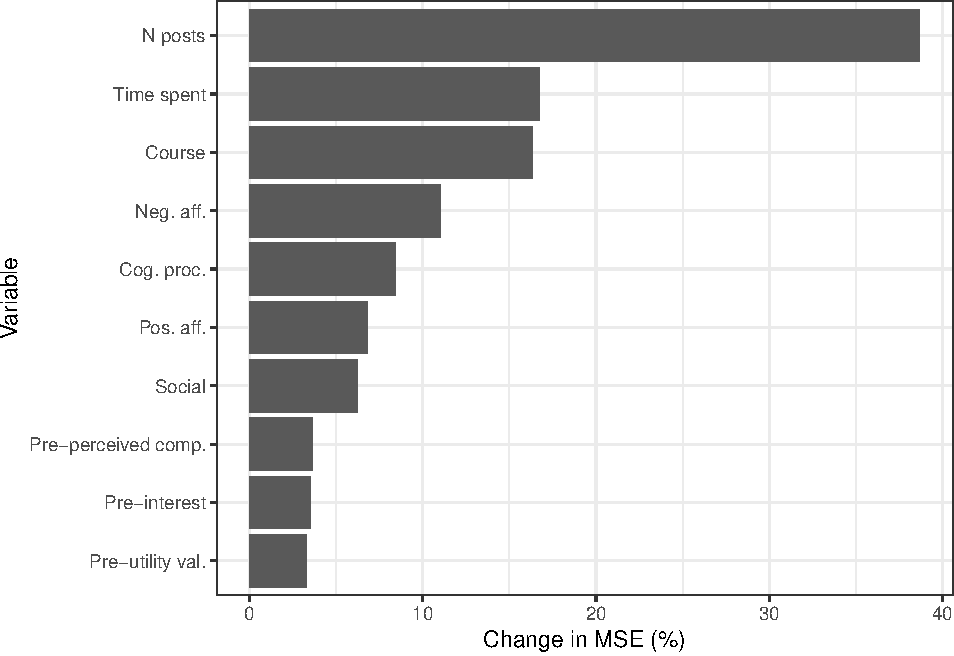
\includegraphics{LAK_Manuscript_blinded_files/figure-latex/unnamed-chunk-3-1.pdf}
\caption{\label{fig:unnamed-chunk-3}Variable importance (change in Mean
Square Error {[}MSE{]})}
\end{figure}

\subsection{Research Question 3}\label{research-question-3}

Research question 3 asked which of the trace variables was most
predictive of course achievement. The most predictive variable in terms
of achievement was the number of posts on the discussion board. This was
the most predictive of all the variables in the model.

\section{4. DISCUSSION}\label{discussion}

Overall, our random forest model explained a large amount of the
variance in achievement in this study (e.g., 55.49\%). However, the
predictive accuracy of the model might ideally be higher: the absolute
value of the average difference between the predicted final grade and
actual final grade was 9.7\%. This discrepancy suggests that whereas our
model did a good job at explaining variance in the outcome of
achievement, it did not perform as well in its prediction of
\enquote{unseen} test data as would be ideal. Future research should
thus explore whether the predictive accuracy of the model could be
further developed. Even so, our predictive accuracy is not so low as to
be unhelpful. Rather, this study offers interesting insights as to the
relative importance of motivation constructs and trace measures of
engagement in terms of explanatory power in explaining middle school
students' online science course grades.

Surprisingly, we found that trace measures of engagement with a learning
management system were more predictive of student achievement than
motivation variables. Past work framed in Expectancy-Value Theory does
not often consider trace measures of engagement, so this is an important
contribution.

\subsection{Limitations}\label{limitations}

This study was limited in some important ways. First, we chose to
operationalize achievement as final course grade. Future work could
examine other meaningful outcomes. Additionally, we did not account for
the number of discussion posts that were required in a given course and
it is important that future research endeavor to explore whether this
plays a role in predicting the outcome.

\subsection{Implications}\label{implications}

As more and more courses move online, data will continue to accumulate
at rapid rates. It is important that educators and administrators
consider the implications of computer-mediated instruction. This study
suggests that the measurement of students' engagement with courses is
helpful in understanding their achievement in these courses. Trace data
is valuable to collect and it could be valuable for educators to
consider it more thoroughly. This study also offers implications in
terms of the motivation constructs studied. The importance of the
engagement with the course through discussion board posts in terms of
predicting final grade suggests that perhaps it is valuable for students
to post even if they are not intrinsically motivated to do so. Future
research should explore the complex relations between student motivation
and course engagement, especially insofar as to examine characteristics
of the online experience that could make these relations different than
the patterns of relations that would be evident in a face-to-face
classroom.

\newpage

\section{References}\label{references}

Allen, I. E. \& Seaman, J. (2008). \emph{Staying the course: Online
education in the United States.} Needham, MA: Sloan Consortium.

Breiman, L. (2001). Random forests. \emph{Machine Learning, 45,} 5--32.
\url{doi:10.1023/A:1010933404324}

Hamilton, L., Halverson, R., Jackson, S., Mandinach, E., Supovitz, J.,
\& Wayman, J. (2009). \emph{Using student achievement data to support
instructional decision making (NCEE 2009-4067).} Washington, DC:
National Center for Education Evaluation and Regional Assistance,
Institute of Education Sciences, U.S. Department of Education. Retrieved
from \url{http://ies.ed.gov/ncee/wwc/PracticeGuide.aspx?sid=12}

Ikemoto, G. S., \& Marsh, J. A. (2007). Cutting through the
\enquote{data driven} mantra: Different conceptions of data-driven
decision making. In P.A. Moss (Ed.), \emph{Evidence and decision making}
(National Society for the Study of Education Yearbook, Vol. 106, Issue
1, pp.~105--131). Chicago, IL: National Society for the Study of
Education.

Liaw, A. (2018). \emph{Package \enquote{randomForest}: Breiman and
Cutler's Random Forests for Classification and Regression.}
\url{https://cran.r-project.org/web/packages/randomForest/randomForest.pdf}

Pennebaker, J.W., Boyd, R.L., Jordan, K., \& Blackburn, K. (2015).
\emph{The development and psychometric properties of LIWC2015.} Austin,
TX: University of Texas at Austin.

\begingroup
\setlength{\parindent}{-0.5in} \setlength{\leftskip}{0.5in}

\hypertarget{refs}{}

\endgroup


\end{document}
